\hspace{1.5cm}The great thing about machine learning is that there are infinite ways to build a model. Even if an algorithm produces results that are considered very valuable, those positive results can always be revamped in unimaginable ways. In some cases, a common and easy way to improve the model is to collect more data to inflate the dataset, which results in nothing more than a better estimation.\\

These cases, where increasing the size of the dataset improves the model obtained, are the cases where overfitting occurs with a significant amount of data.

\section*{Learning Curves}
As mentioned in the learning curves section (2.3.1), plotting as a function of training set size can be very useful for estimating progress as more observations are added to the data. Ridge regression proved to be underfitting (which was to be expected since it is a simple linear model), but plotting the learning curves for Random Forest yields Figure 4.1. Clearly, overfitting is observed, the training error remains relatively small, while the test error appears unreasonably high.
\begin{figure}
    \centering
    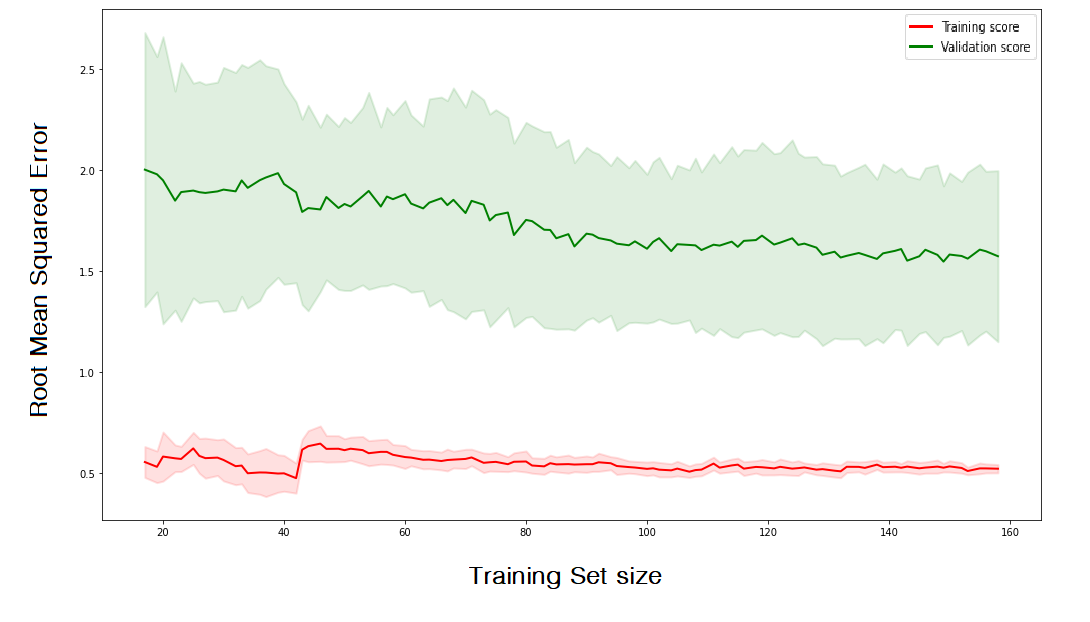
\includegraphics[width=0.6\textwidth]{Images/Discussion/Learningcurve.png}
    \caption{Learning curves for Random Forest with respect to the training set size.}
\end{figure} 

The trends toward lower test error are not clear in the graph, but they are there. Perhaps not in the case where 500 more molecules are added to the dataset, but if the observations of a million molecules, which is not unusual in this respect, were available for training the model, a significant decrease in test error would be seen. Collecting data is usually a rather mechanical process, not very difficult but tedious to do by hand. In this model, the estimation would not have been much better if the size of the dataset had been doubled, but the actual size provides insight into the overfitting that exists and what needs to be done if improvement is intended.\\\\

Sometimes, the opposite action, selectively removing those considered non valuable observations, is another option. More than the non-valuable observations, the clusters where the error is too high can be examined to find the reason. This can be taken further using cluster error analysis.
\section*{Cluster Based Error Analysis}
With respect to what should the observations be clustered? Descriptors can be chosen, or even the response feature. Another valuable option is using the molecular fingerprints as the criterion.
\subsection*{Molecular Fingerprints}
To calculate fingerprints for a series of molecules, it is necessary for the dataframe to have a column describing the \textbf{SMILES} chains of the molecules. SMILES chains describe the structure of a molecule in a simplified form, with all its atoms (except for hydrogen) and the types of bonds between them. An example would be, glucose: C([C@@H]1[C@H]([C@@H]([C@H](C(O1)O)O)O)O)O . But how to arrive at clusters starting with these identifiers? From these SMILES chains, a conventional 1024-bit fingerprint is created for each molecule. This fingerprint can be represented as a 1024-dimensional vector with ones and zeroes. Each 1 would refer to the existence of a substructure determined in the algorithm. This vector is now viable to be a clustering criterion.\\

K-fold clustering was carried on, and k=11 was used. In Figure 4.2 are 8 of the 22 molecules in the first cluster where conformation similarities can be clearly spotted.
\begin{figure}[h!]
    \centering
    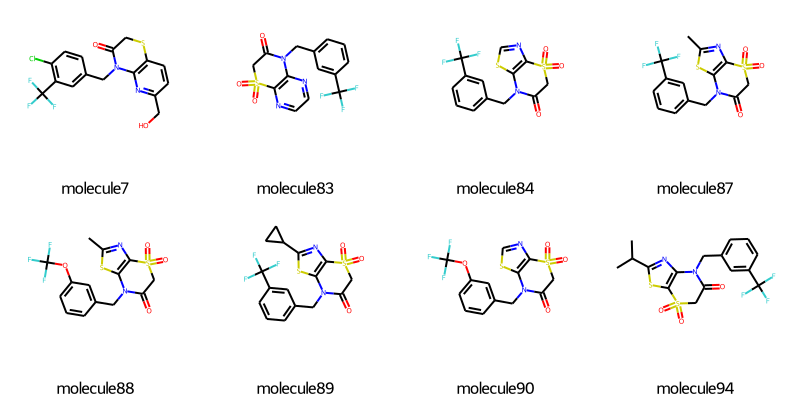
\includegraphics[width=0.7\textwidth]{Images/Discussion/clusterfinger.png}
    \caption{Molecules corresponding to Cluster 1 after carrying out k-fold clustering in molecular fingerprints.}
\end{figure}

The errors in each cluster vary as it can be perceived in Figure 4.3.
\begin{figure}[h]
    \centering
    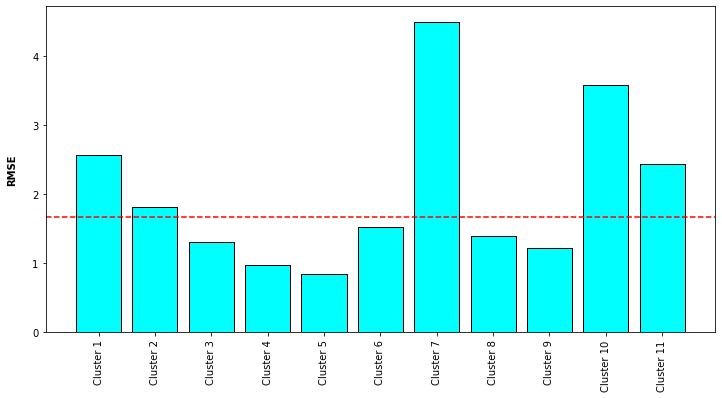
\includegraphics[width=0.8\textwidth]{Images/Discussion/clustererror.png}
    \caption{Error found in each cluster in Random Forest.}
\end{figure}


\section*{Metaregressors}
When it comes to the algorithm itself and the choice of making to solve for this problem, even if Random Forest was a good choice, there is no perfect regressor, and the option can be improved to get even better results.\\

The better half of this problem resides in metaregressors, which are ensembles of algorithms such as Random Forest and Support Vector Machines. These metaregressors are designed to optimize even further in expense of computation, they are very promising.\\\\\\\\\\\\\\



\section*{Conclusion}
In conclusion, a larger hereness of molecule data or the creation of a database with a large number of molecules could significantly improve the model; and not only that, the application of a metaregressor combined with this could potentially refine a huge lot the results obtained. Even with all this said, the Random Forest algorithm performed very well and deserves the credit granted.